\chapter{Especificação e Metodologia} \label{chp:espec_metodologia}

\section{Divisão do Projeto}
O projeto pode ser dividido em dois sub-projetos, cada qual lidando com um objetivo listado na seção anterior. O primeiro sub-projeto tem a finalidade de estruturar uma \textbf{rede de sensores} e atuadores utilizando um protocolo aberto a ser desenvolvido neste trabalho, a fim de atingir o objetivo i. O segundo sub-projeto busca desenvolver um \textbf{serviço em nuvem} que agregue os dados coletados pela rede de sensores, efetuando, entre outras atividades, o processo de aprendizagem descrito no objetivo ii.

O primeiro passo na especificação consiste na identificação dos \textit{stakeholders}. Em seguida, a especificação do projeto será feita por meio de requisitos funcionais e não-funcionais, que estão listados em três classes:
\begin{itemize}
	\item Requisitos de sistema, relativos à integração de ambos os sub-projetos;
	\item Requisitos da rede de sensores, referente ao sub-projeto dedicado a atingir o objetivo i; 
	\item Requisitos do serviço em nuvem, referente ao sub-projeto dedicado a atingir o objetivo ii.
\end{itemize}

\section{Descrição dos \textit{stakeholders}}
Os seguintes \textit{stakeholders} foram identificados no projeto:
\begin{itemize}
	\item Usuário final, cujo interesse seria adquirir e instalar dispositivos em sua residência, de modo a obter automação residencial. Um perfil possível para este tipo de stakeholder seria uma pessoa com conhecimento técnico básico em computação e redes de computadores. Ele deve ser capaz de conectar os dispositivos na rede desejada (por exemplo, na rede Wi-Fi por onde todo o tráfego deve passar), mas os demais procedimentos de estruturação da rede de sensores segundo o protocolo devem ser feitos de forma transparente;
	\item Desenvolvedor, cujo interesse seria estudar a documentação dos protocolos e algoritmos desenvolvidos, e projetar dispositivos compatíveis. Este stakeholder seria usuário das bibliotecas (APIs) resultantes do projeto. Ele espera encontrar documentos explicando o funcionamento dos protocolos e dos algoritmos desenvolvidos, bem como documentações e exemplos de uso das APIs que deve utilizar. Ainda, estes desenvolvedores consideram como diferencial o fato de a licença de uso das tecnologias disponibilizadas serem abertas e isentas de pagamento.
\end{itemize}

\section{Requisitos Funcionais} \label{sec:reqfunc}
\subsection{De sistema}
\begin{itemize}
	\item O sistema deve coletar dados do ambiente domiciliar e possibilitar a ativação de atuadores automaticamente ou por ação humana;
	\item O sistema deve permitir que o usuário visualize o estado atual do sistema;
	\item O sistema deve se adaptar a alterações de gostos e preferências do usuário.
\end{itemize}

\subsection{Da rede de sensores}
\begin{itemize}
	\item Toda a comunicação deve ser realizada através de um protocolo único e formalizado;
	\item O protocolo de comunicação deve permitir a identificação dos dispositivos da rede, bem como o envio de dados e de comandos de atuação.
\end{itemize}

\subsection{Do serviço em nuvem}
\begin{itemize}
	\item Permitir acesso remoto em qualquer localização para que usuário controle seus dispositivos à distância;
	\item Aprender os hábitos do usuário e configurar a rede de sensores automaticamente para realizar os seus gostos.

\end{itemize}

\section{Requisitos Não-Funcionais} \label{sec:reqnfunc}
\subsection{De sistema}
\begin{itemize}
	\item Fácil instalação de sensores e integração com a nuvem;
	\item Utilizar linguagens, ambientes e bibliotecas abertas.
\end{itemize}

\subsection{Da rede de sensores}
\begin{itemize}
	\item O protocolo de comunicação desenvolvido deve ser aberto, de modo que qualquer fabricante possa criar um dispositivo que compatível com a rede;
	\item Deve possibilitar o uso de diversas tecnologias de comunicação, tais como ZigBee, IEEE 802.15.4, e UDP;
	\item O protocolo deve gerar pacotes de tamanhos compatíveis com tecnologias de redes existentes para redes de sensores sem fio;
	\item A rede deve continuar operante mesmo sem acesso à nuvem.
\end{itemize}

\subsection{Do serviço em nuvem}
\begin{itemize}
	\item Disponibilidade de 99,9\% do tempo (no máximo 8h/ano indisponível); 
	\item API que possibilite o acesso através de aplicações de terceiros, aplicativos móveis ou \textit{websites}.
\end{itemize}

\section{Limitações e Suposições}
Os itens elicitados a seguir não fazem parte do escopo do sistema e podem ser abordados em trabalhos futuros.

\subsection{Da rede de sensores}
\begin{itemize}
	\item Conectividade: o protocolo desenvolvido supõe que os dispositivos já estejam conectados a uma rede comum e confiável. Maiores detalhes presentes na seção \ref{subsec:limit_conectividade};
	\item Segurança: o protocolo desenvolvido supõe que a infraestrutura de rede subjacente seja segura, e que os nós pertencentes à rede de sensores e atuadores sejam confiáveis. Maiores detalhes presentes na seção \ref{subsec:limit_seguranca}.
\end{itemize}

\subsection{Do serviço em nuvem}
\begin{itemize}
	\item Segurança: a comunicação entre dispositivos é feita de forma aberta neste projeto, como explica a seção \ref{subsec:limit_serv_app};
	\item Dependência de conexão à internet: a interação do usuário com o sistema por meio do aplicativo depende de conexão à internet, como explica a seção \ref{subsec:limit_serv_app};
	\item Processo de aprendizagem: neste projeto, o objetivo proposto foi de implementar um processo de aprendizagem para um domínio específico, mostrando a viabilidade de aplicar tais algoritmos para prover automação residencial. Assim sendo, o processo implementado possui diversas limitações, levando-se em conta a aplicação em um sistema real de automação residencial. A seção \ref{subsec:limit_aprendizgem} explica em detalhes tais limitações.
\end{itemize}

\section{Arquitetura do Sistema} \label{sec:arquitetura}
Seguindo a descrição apresentada do projeto, o grupo definiu a arquitetura do sistema de automação residencial conforme mostra a Figura \ref{fig:arquitetura}.

\begin{figure}[h]
	\centering
	\caption{Arquitetura do sistema de automação residencial.}
  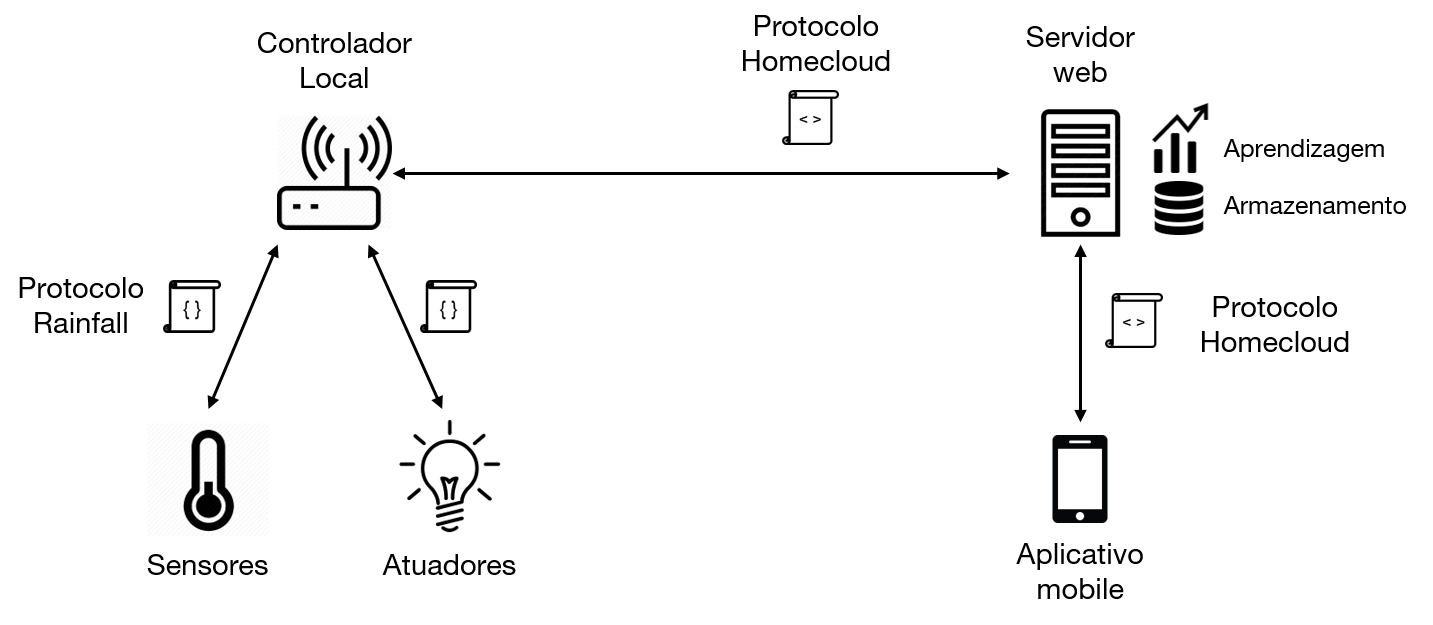
\includegraphics[width=\textwidth]{imagens/arquitetura.png}
  \label{fig:arquitetura}  
\end{figure}

A arquitetura contém dispositivos sensores e atuadores, que efetuam a coleta de dados nas residência e atuam nelas. Esses dispositivos se comunicam com um controlador local, que efetua o gerenciamento dos nós locais (a aceitação de nós na rede, por exemplo) e a interface entre os dispositivos locais e a infraestrutura em nuvem. A comunicação entre os dispositivos mencionados é feita por meio do protocolo Rainfall, desenvolvido e especificado neste projeto. O desenvolvimento desses dispositivos e do protocolo mencionado serão o foco do primeiro sub-projeto.

Além disso, constam no diagrama um servidor em nuvem e um serviço de armazenamento e análise de dados. O servidor em nuvem atua como um agregador dos dados coletados pelos diversos controladores locais. Sobre este banco de dados, o serviço de análise (mineração de dados e aprendizagem de máquina) atuará no sentido de derivar padrões de comportamento dos usuários, sugerindo regras de automação residencial. Por fim, aponta-se a existência de um elemento de interface gráfica com a qual o usuário pode interagir com o sistema, representado na arquitetura apresentada como um \textit{smartphone}. O elemento de interface com o usuário se comunica com o servidor em nuvem, e pode eventualmente se comunicar com o controlador local. A comunicação entre o servidor e os demais componentes (controlador local e aplicativo móvel) é feita por meio do protocolo Homecloud, também desenvolvido e especificado neste trabalho. Tais componentes da arquitetura serão foco do segundo sub-projeto.

O diagrama mostrado na Figura \ref{fig:arquitetura_uml} apresenta uma visão em camadas da arquitetura. Para este projeto, adotou-se um modelo em três camadas, quais sejam a de fronteira, de negócios e de dados. 

\begin{figure}[h]
	\centering
	\caption{Arquitetura em camadas do sistema de automação residencial.}
  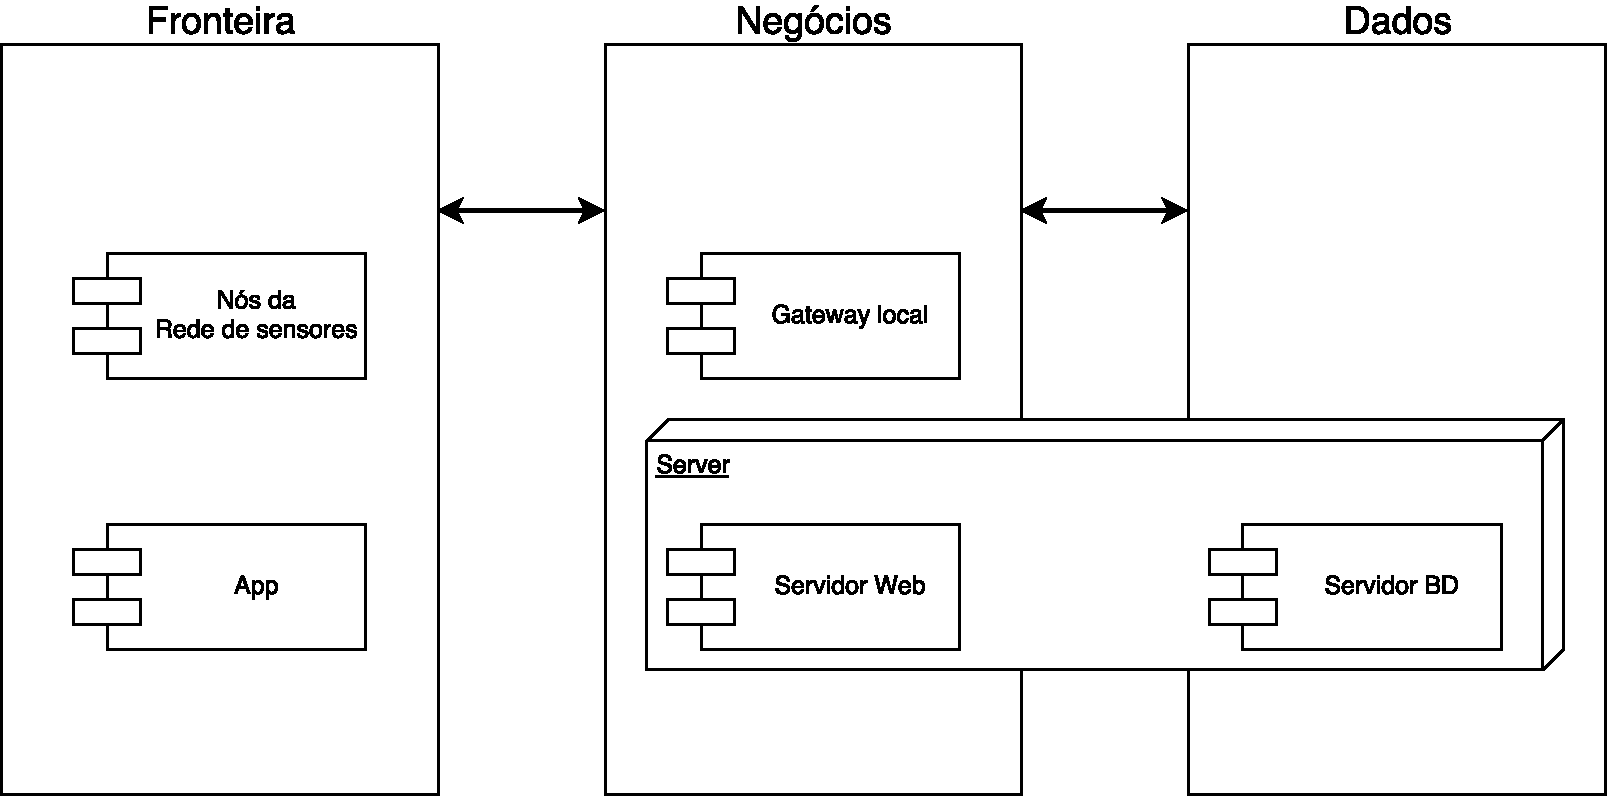
\includegraphics[width=\textwidth]{imagens/arquitetura_uml.pdf}
  \label{fig:arquitetura_uml}  
\end{figure}

A camada de fronteira engloba elementos que interagem com o ambiente ou com os atores do sistema. Os dispositivos da rede local (sensores e atuadores), bem como o aplicativo móvel, compõem esta camada. A camada de negócio contém as funcionalidades ou lógica de negócio, não possuindo interface para os atores nem persistência de dados. Esta camada é composta pelo controlador ou \textit{gateway} local e pelo servidor \textit{web}. Por fim, a camada de dados é responsável pela persistência dos dados utilizados nas demais camadas, e é composta pelo servidor de banco de dados.

O diagrama mostra ainda um aspecto de implementação física do projeto, que é o agrupamento do servidor \textit{web} e do servidor de banco de dados. No presente projeto, estes servidores serão executados em um mesmo equipamento em nuvem.

\section{Metodologia} \label{sec:metodologia}
O grupo utilizou princípios da metodologia Scrum para nortear o desenvolvimento do projeto. O Scrum é uma metodologia ágil de desenvolvimento de projetos iterativo e incremental, prevendo a volatilidade de requisitos, pregando a rápida disponibilização de produtos entregáveis ao cliente \cite{schwaber2016}.

Um dos conceitos fundamentais do Scrum são os \textit{sprints}, definido como um período de trabalho de um mês ou menos em que um produto entregável pode ser desenvolvido e disponibilizado. Um projeto consiste de diversos \textit{sprints} executados de forma sucessiva, razão pela qual diversos produtos intermediários (mas utilizáveis) são gerados neste processo.

O grupo utilizou extensivamente este conceito de \textit{sprints} para gerenciar o desenvolvimento do projeto. Para tanto, foi utilizada a plataforma Trello\footnote{Disponível em \url{https://trello.com/}.}, que permite organizar as \textit{sprints} planejadas e os itens de trabalho pendentes, em execução e finalizados (Figura \ref{fig:interface_trello}).

\begin{figure}[h]
	\centering
	\caption{Interface da plataforma Trello.}
  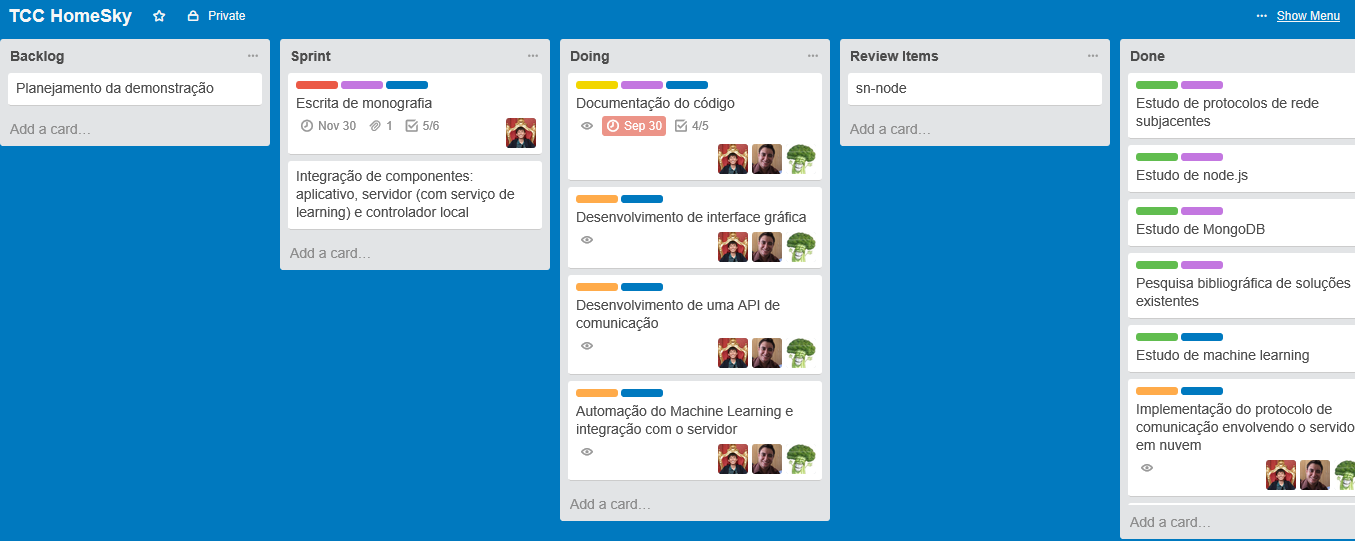
\includegraphics[width=\textwidth]{imagens/interface_trello.png}
  \label{fig:interface_trello}  
\end{figure}

Além disso, o grupo adotou diversas práticas recomendadas pelo PMBOK no que tange à gestão de escopo e de tempo do projeto \cite{pmbok}. Em primeiro lugar, foi especificado a Estrutura Analítica do Projeto (EAP - ver Figura \ref{fig:eap}), listando os itens tangíveis e verificáveis produzidos como resultado do projeto. Com base na EAP, foi possível definir as atividades do projeto e definir o cronograma de atividades. Este cronograma foi utilizado para definir as \textit{sprints} a serem seguidas no decorrer do trabalho.

\begin{figure}[h]
	\centering
	\caption{Estrutura Analítica do Projeto.}
  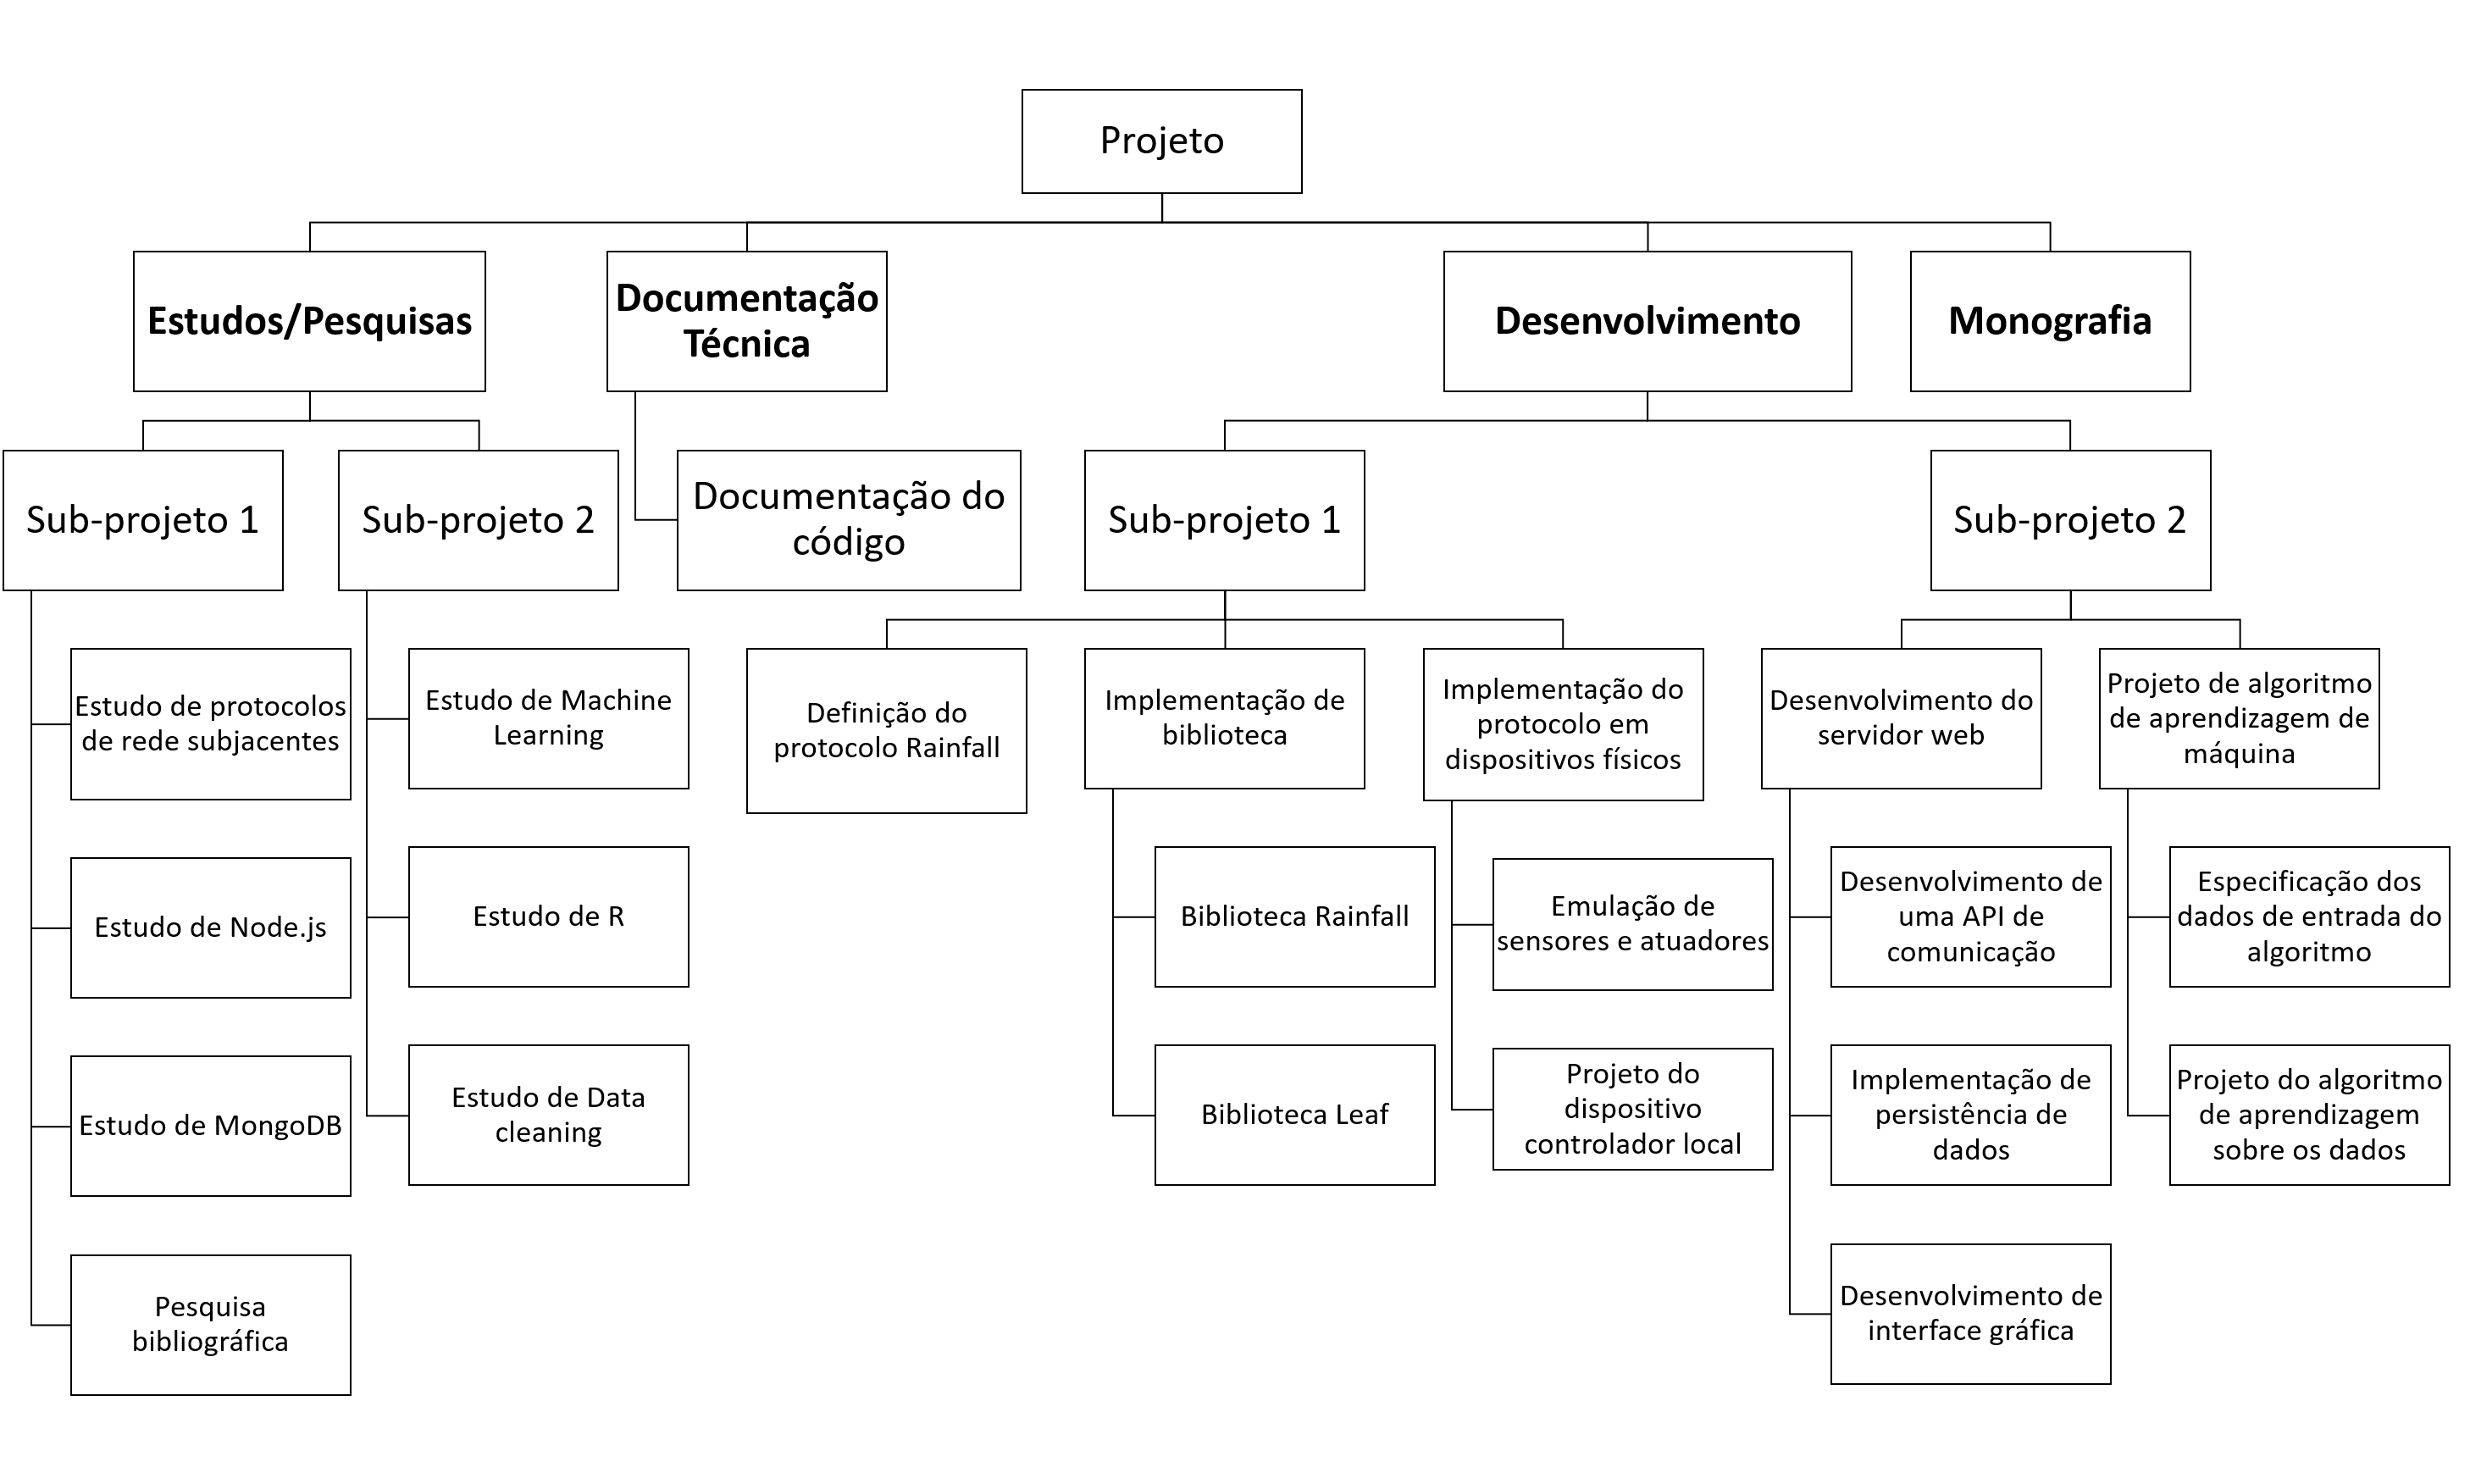
\includegraphics[width=\textwidth]{imagens/eap.png}
  \label{fig:eap}  
\end{figure}
